\section{\color{Red}A Zoo of Monoids}


We have seen that $\Mon{\nats}{+}{0}$, $\Mon{\nats}{\times}{1}$, and $\Mon{\nats}{+_{12}}{12}$ are monoids. Square matrices of whole numbers under matrix multiplication also form monoids. We can devise many more such numerical examples, but the monoids of interest to data professionals are the ones that represent collections. Let us define a list structure and show the monoidal structure:
\begin{definition}
  A \textbf{list} is an ordered sequence of zero or more items of some type $\T$. A monoid of lists has the associative, non-commutative, binary operation, $\pp$, for concatenating lists and the empty list as identity.
  \label{def:list}
\end{definition}


As defined, a set of lists can be a monoid! The definition is a bit austere, though: we need notation. Write the empty list as $\emptylist$ and the general list as $[a_1, a_2, \ldots]$, making sure that every element $a_i$ is of the same type, that is, is an element of $\T$. Write that last assertion symbolically as $\forall i,a_i \in \T$, reading ``$\forall$'' as ``for all'' and ``$\in\,$'' as ``in'' or ``is an element of.'' The term \textbf{ordered} means that we only need to know a number or \textbf{index} $i$ to find an element $a_i$ of the list. Later, we encounter some unordered monoids, wherefrom we \emph{cannot} find an element given only its index.


The indices $i$ come from the natural numbers excluding zero, written \mbox{$\nats-\{0\}$}. This is \emph{1-based indexing} and is the usual convention in mathematics. Occasionally, it is more convenient to start indices at 0, drawing them from all of $\nats$, writing the general list as $[a_0, a_1, \ldots]$. This is \emph{0-based indexing}, is an equally valid convention to 1-based indexing, and is the norm for programming languages.


We might have defined list monoids without restricting their items to come from a type set $\T$. For instance, we might want a list to contain both integers and ASCII characters, or nested lists. That sort of definition is called a \emph{heterogeneous list}, like lists in the programming language Lisp. However, such is a bit out of vogue nowadays, partly due to the ascendence of strongly typed programming languages and partly due to applications to relational databases to follow. On balance, it is beneficial to name and restrict the types of elements that a particular list may contain.


The empty list as identity means that $\mathcal{L}\pp\emptylist=\mathcal{L},\; \emptylist\pp\mathcal{L}=\mathcal{L}$
for any list $\mathcal{L}$.


Now, consider a couple of particular lists of integers, say $\mathcal{L}_1=[6,7,8]$ and $\mathcal{L}_2=[4,5]$. Invoke the operation and construct
\begin{align*}
  \mathcal{L}_1 \pp \mathcal{L}_2 &= [6,7,8,4,5] \\
  \mathcal{L}_2 \pp \mathcal{L}_1 &= [4,5,6,7,8]
\end{align*}
\begin{observation}
  Lists and $\pp$ are not commutative.
\end{observation}


Is every set of lists a monoid? No. Consider the set of lists of no more than three integers. By concatenating suitably large elements of this set, we get lists of more than three integers, thus, the set is not closed under concatenation, and is therefore not a monoid.


But also consider the set of lists of integers where the first element of every list is the number 1. This set \emph{is} a monoid, since there is no way to get rid of an initial 1 by concatenation! Concatenate a list beginning with a 1 to either the front or the back of a list beginning with a 1 and you will still have a list beginning with a 1. The identity element is the empty list. The first element of the empty list is a 1 by a strange but valid technicality of logic. I cannot show you any element of the empty list that is \emph{not} a 1, therefore, the statement that the first element of the empty list is a 1 must be correct. It is impossible to prove it false, and the Law of the Excluded Middle insists that it be either true or false.


Imagine a dictionary of words considered as lists of characters. The entire dictionary might be a list monoid, and by analogy to the monoid of lists of integers with first element 1 above, each alphabetical section might also be a list monoid, but there is a stipulation. Each alphabetical section must, in fact, be infinite in length, just as must be the entire dictionary, since, given any two words, I can always create a longer word by concatenating the two. Even though each entry in the dictionary is finite in length, the entire dictionary is infinite in length, and so, in fact, is every subsection of the dictionary. Redefine a dictionary subsection to mean ``the set of words with any finite prefix whatever.'' So, the `a's form one subsection, as before, but so do the `aa's and the `ab's and the `qu's and the `str's and so on. This is the kind of dictionary that Jorge Luis Borges might have liked \cite{babel}.\footnote{Borge's library consisted of 410-page books of 40$\times$80 lines, from a 25-character alphabet. There are $25^{40\times 80\times 410}\approxeq1.96\times 10^{1,834,097}$ different such books. While a fairly large number, this is, existentially finite.}


The trivial list monoid contains just the empty list and no other lists. No other list monoid can be finite under concatenation, since, given any two elements, we can always create another, longer element. Even the monoid of lists of just 1's contains the elements $\emptylist$, $[1]$, $[1,1]$, and so on, without end.


There is an alternative, recursive definition for list, equivalent in every way to definition \ref{def:list}, above, but perhaps more familiar to programmers:
\begin{definition}
  A \textbf{list} of elements of type $\T$ is either the empty list or a singleton $[a]$ concatenated to a list, where $a\in \T$.
  \label{def:recursivelist}
\end{definition}
A \textbf{singleton} is just a list containing a single element. A better way of writing this is in BNF (Backus-Naur Form):
\begin{center}
  \begin{tabular}{crll}
    \emph{List}$\langle \T\rangle$  &  $\bnfisa$  &  $\emptylist$
      & \emph{a list of elements of type $\T$ is either the empty list}\\
    \mbox{}  &  $\vert$  &  $[a\in\T]\pp$ \emph{List}$\langle \T\rangle$
      & \emph{or a singleton concatenated to another list}\\
  \end{tabular}
\end{center}
emphasizing that $a\in \T$.


%Shorten the notation by writing \mbox{\emph{List}$\langle \T\rangle$} as just $[\T]$, yielding
%\[  [\T] \bnfisa \emptylist \;\; \vert \;\; [a\in \T] \pp [\T]  \]


As before, write the monoid as $\Mon{\T}{\pp}{\emptylist}$. The interesting bit is the first slot, the type set of the monoid, $\T$. The recursive version of the definition reveals that lists are built from singletons of the form $[a]$ rather than directly from elements of $\T$. Does this technical detail call into question our definition of a monoid, definition \ref{def:monoid}? There, we wrote that a monoid is a set of elements `of type $\T$.' There is just enough wiggle room to accommodate lists as elements of a monoid if we allow `of type $\T$' to mean `elements of the set $\T$ or elements of the set of singleton lists made from elements of the set $\T$.' Let us write this latter set, the set of singleton lists, as $[\T]$ for short. Each element of this latter set is a special kind of element of the monoid of lists. We convert elements of the monoid's type set $\T$ into the derivative type set $[\T]$ before they can participate in the monoid. We must introduce an auxiliary operation, called \textbf{unit}, that just takes an arbitrary element of $\T$ and returns a singleton. Symbolize \emph{unit} for lists as $\mathcal{U_{\emptylist}}$, and denote the fact that it maps elements of the type set $\T$ to singleton elements of the monoid as follows:
\begin{center}
  \begin{tabular}{ll}
    $\mathcal{U_{\emptylist}}:\T\rightarrow[\T]$ & \emph{$\mathcal{U_{\emptylist}}$ maps elements of $\T$ to elements of $[\T]$}\\
    $\forall a\in \T, \mathcal{U_{\emptylist}}(a)=[a]$ & \emph{for any $a$ in $\T$, $\mathcal{U_{\emptylist}}(a)$ is the singleton $[a]$}
  \end{tabular}
\end{center}


\subsection{\color{Red}Where was the Unit?}


We didn't have to go through all this with the numerical monoids $\Mon{\nats}{+}{0}$ and $\Mon{\nats}{\times}{1}$, or even with the more complicated monoid of square matrices. What gives? Why is this different? The answer is that we actually did go through all this with the numerical monoids, just under the covers, without talking about it. Now we must.


Revisit the clock-arithmetic example, $\Mon{\nats}{+_{12}}{12}$, the monoid of whole numbers under addition modulo 12. Now we can see that we confused the type set, $\nats$, and the set of `singleton' elements of the monoid, which really must be the finite set $\{1,2,\ldots,12\}$, henceforth written $\nats_{12}$. There were no consequences to the confusion because this monoid contains \emph{only} singleton elements and because the unit function is so trivial in this case. The list monoid, though, has shown us that, in general, we must map type-set elements into singletons, so now we must go back and reconsider all the prior examples and identify those unit functions.


Before an element of $a\in\nats$ can participate in the clock-arithmetic monoid, $a$ must undergo conditioning --- be tweaked --- be brought into the set of singletons, $\nats_{12}$, by computing its residual mod 12, that is, its remainder when divided by 12. So, the unit function for $\Mon{\nats}{+_{12}}{12}$ is
\begin{center}
  \begin{tabular}{l}
    $\mathcal{U}_{12}:\nats\rightarrow\nats_{12}$\\
    $\forall a \in \nats, \mathcal{U}_{12}(a)=a \bmod 12$\\
  \end{tabular}
\end{center}
Even the monoids $\Mon{\nats}{+}{0}$ and $\Mon{\nats}{\times}{1}$ have unit functions:
\begin{center}
  \begin{tabular}{lcl}
    $\mathcal{U}_{+,0}:\nats\rightarrow\nats$ & \rule{5ex}{0ex} &
    $\mathcal{U}_{\times,1}:\nats\rightarrow\nats$ \\
    $\forall a \in \nats, \mathcal{U}_{+,0}(a)=a$ & \rule{5ex}{0ex} &
    $\forall a \in \nats, \mathcal{U}_{\times,1}(a)=a$\\
  \end{tabular}
\end{center}


All these unit functions are pretty trivial, but these last ones are about as trivial as it gets: they just return their arguments without change. The function that does such is called \emph{id}, the \textbf{identity function}, not to be confused with the identity \emph{element} of a monoid. It is useful to symbolize this function in \textbf{lambda notation}. Read $\lambda x$ as ``the function of $x$ that\ldots'':
\begin{center}
  \begin{tabular}{ll}
    $\mathrm{id}=\lambda x.x$, & \emph{\textbf{id} is the function of $x$ that returns $x$ for any $x$}\\
  \end{tabular}
\end{center}


The point is that every monoid must have a unit function to convert elements of the type set $\T$ into singleton elements of the monoid. We \emph{might}, at this point, force ourselves to be so pedantic as to rewrite every monoid with its unit function and set of singletons, like this:
\[ \mathcal{M}\langle\nats,\lambda x.(x\bmod 12),\nats_{12},+_{12},12\rangle \]
But that is really going too far, because, although the unit function and sets of singletons \emph{exist} for every monoid, they are so trivial that usually we just need to note them once and then forget them. They are a little like the door to a house: not, by any means, the most interesting part of the house, and not worth talking about at all once one has passed through it. But it is an essential part. Later, we find that careful accounting for \emph{unit} leads us from monoids to monads, their practical cousin in programming languages.


\subsection{\color{Red}The Collection Monoids}


Lists are our first example of a \textbf{collection monoid}. There are three other kinds: \emph{set}, \emph{bag}, and \emph{permutation}.\footnote{my friend, Carl Kelso, coined the term \emph{suit} for such monoids; this is altogether a more suitable name because it is a monosyllable, like the other three names, it directly invokes the correct intuition from playing cards, and it is less technically fearsome than \emph{permutation}.} They differ in whether they are ordered and whether they are \emph{idempotent}, and that is why there are just four: two choices for `ordered or not' and two, independent choices for `idempotent or not.' We have already explained the concept of \emph{ordered}. Let us define idempotent:
\begin{definition}
An operation, $\oplus$, is \textbf{idempotent} if $x\oplus x=x$ for any $x$ in the domain of $\oplus$.
\label{def:idempotentoperation}
\end{definition}
\begin{definition}
A collection is \textbf{idempotent} if no duplicate elements are allowed.
\label{def:idempotentcollection}
\end{definition}


We see below that idempotency of an operation does not suffice, in general, to guarantee idempotency of a collection. So, the two definitions, while related, are distinct.


A list monoid is neither commutative nor idempotent, so, in some sense, it is the simplest of the four kinds. A \emph{permutation} monoid is idempotent and non-commutative. Consider the ordered sequence $\pmx{1, 2, 3}$. Because it is ordered, it is distinct from $\pmx{2, 1, 3}$, and, in fact, from all four other permutations or orderings of the numbers 1, 2, and 3. Because $\pmx{1, 2, 3}$, as a permutation, is idempotent, we cannot add, prepend, or append another copy of 1, 2, or 3 to it.


\begin{trial}
  A \textbf{permutation} is an ordered sequence of zero or more items of some type $\T$. A monoid of permutations has the associative, non-commutative, idempotent, binary operation, $\boxplus$ (pronounced `box-plus'), for concatenating permutations, and the empty permutation, $\emptyperm$ (pronounced `bananas'),\footnote{It is with some regret that I use banana brackets for permutations, since Meijer, Trust, and others use them for catamorphisms. However, I was not able to find another viable bracket form for permutations amongst the mutually compatible font sets I have at hand.} as identity.
\end{trial}


As stated, a collection of permutations can be a monoid, but we must be more precise concerning idempotency. The first task is to `design' $\boxplus$: to write out its operational rules and see if we can build with it a collection that contains no duplicate elements. Let $s$ and $t$ be distinct elements of $\T$, and let $\emptyperm$ be the empty permutation. Write the type of \emph{permutations of items of type $\T$} as $\LPerm\T\RPerm$. The unit function will map elements of $\T$ to singleton elements of $\LPerm\T\RPerm$:
\begin{center}
\begin{tabular}{ll}
  $\mathcal{U}_{\LPerm\RPerm}:\T\rightarrow\LPerm\T\RPerm$ &
  \emph{$\mathcal{U}_{\LPerm\RPerm}$ maps elements of $\T$ to elements of
  $\LPerm\T\RPerm$}\\
  $\forall s \in \T, \mathcal{U}_{\LPerm\RPerm}(s)=\LPerm s\RPerm$ &
  \emph{for any $s$ in $\T$, $\mathcal{U}_{\LPerm\RPerm}(s)$ is the singleton $\LPerm s\RPerm$}\\
\end{tabular}
\end{center}


Now, build up some base cases. We want $\boxplus$ to satisfy the following equations.
\begin{align}
  \nonumber
  \LPerm s \RPerm \boxplus \emptyperm &= \LPerm s \RPerm \\
  \nonumber
  \emptyperm \boxplus \LPerm s \RPerm &= \LPerm s \RPerm \\
  \nonumber
  \LPerm s \RPerm \boxplus \LPerm t \RPerm  &= \LPerm s, t \RPerm \\
  \nonumber
  \LPerm t \RPerm \boxplus \LPerm s \RPerm  &= \LPerm t, s \RPerm
\end{align}
Since permutations are ordered, then \mbox{$\LPerm s, t \RPerm\neq\LPerm t, s \RPerm$} when $s\neq t$:
\begin{observation}
  Permutations are not commutative and $\boxplus$ is not commutative.
\end{observation}
just as with lists. Still working with singletons, we want
\[ \LPerm s \RPerm \boxplus \LPerm s \RPerm = \LPerm s \RPerm \]
This is idempotency of $\boxplus$, but it is not quite enough to guarantee no duplicates in an arbitrary permutation. So far, we only know (1) how to deal with the identity element and (2) how to create doubletons from singletons. We do not know how to apply $\boxplus$ to an element like $\LPerm s, t\RPerm$ with more than one item in it. There are several ways to proceed, but let us try the recursive style, just as with lists:
\begin{trial}
  A permutation $\mathcal{P}$ of elements of type $\T$ is either the empty permutation $\emptyperm$ or a singleton permutation, $\LPerm s\RPerm$, where $s\in\T$, associatively, non-commutatively, and idempotently concatenated to another permutation, that is, \mbox{$\mathcal{P}_1=\pmx{s}\boxplus \mathcal{P}_2$}.
\end{trial}


Now, consider an arbitrary non-empty permutation, \mbox{$\LPerm s, t, \ldots\RPerm$=$\LPerm s \RPerm \boxplus \mathcal{P}$}, and try to concatenate $\LPerm s\RPerm$ to it. Due to associativity and binary idempotency, we get
\begin{align*}
   \LPerm s\RPerm \boxplus \left\lgroup \LPerm s \RPerm   \boxplus \mathcal{P}\right\rgroup  &=
  \left\lgroup \LPerm s\RPerm \boxplus  \LPerm s \RPerm \right\rgroup \boxplus \mathcal{P} \\
  &= \LPerm s \RPerm   \boxplus \mathcal{P}
\end{align*}
So, adding an element $\LPerm s\RPerm$ to the front of a permutation $\mathcal{P}$ that already has $\LPerm s\RPerm$ at the front does not change $\mathcal{P}$. But suppose $\LPerm s\RPerm$ is buried inside $\mathcal{P}$. Nothing in the design of $\boxplus$ so far prevents us from building, say, $\LPerm s, t, s\RPerm$, which would have an unacceptable duplicate element. We must conclude:
\begin{observation}
  Idempotency of an operation does not guarantee idempotency of a collection.
\end{observation}


We are forced to redesign $\boxplus$. Write the arbitrary finite permutation of length $n\ge 1$ as $\mathcal{P}$=$\LPerm s_1, s_2, \ldots, s_n\RPerm$, where all the $s_i$ are distinct, that is, no two of the elements are equal to one another. Now concatenate a singleton permutation, $\LPerm s\RPerm$, to the front or back of $\mathcal{P}$:
\begin{align}
  \LPerm s\RPerm \boxplus  \LPerm s_1, s_2, \ldots, s_n\RPerm &=
  \begin{cases}
    \LPerm s_1, s_2, \ldots, s_n\RPerm &
      \text{if $s$ equals any of the $s_i$, $i=1$ to $n$},\\
    \LPerm s, s_1, s_2, \ldots, s_n\RPerm &
      \text{if $s$ equals none of the $s_i$}.
  \end{cases}  \label{eqn:recursivelyidempotent1} \\
  \LPerm s_1, s_2, \ldots, s_n\RPerm  \boxplus \LPerm s\RPerm &=
  \begin{cases}
    \LPerm s_1, s_2, \ldots, s_n\RPerm &
      \text{if $s$ equals any of the $s_i$, $i=1$ to $n$},\\
    \LPerm s_1, s_2, \ldots, s_n, s\RPerm &
      \text{if $s$ equals none of the $s_i$}.
  \end{cases} \label{eqn:recursivelyidempotent2}
\end{align}
If the starting permutation $\mathcal{P}$ has no duplicates, the rules above make it impossible for there \emph{ever} to be any duplicates, since $\boxplus$ does not change $\mathcal{P}$ in that case.


The two rules above let us concatenate singletons to the front or to the back of any permutation. Letting $n=1$ and $s_1 =s$ in the above shows the new $\boxplus$ is an idempotent operation, under definition \ref{def:idempotentoperation}, that also preserves the idempotency of a permutation. But it is not yet complete as the operation of a permutation monoid, because it can only concatenate singletons to elements of a monoid. Fixing this is the final detail in the new design of $\boxplus$. First, to see pointedly why it needs fixing, which of the following two is true when $s\neq t$?
\begin{align}
  \LPerm s, t \RPerm \boxplus \LPerm t, s \RPerm &= \LPerm s, t \RPerm
  \label{eqn:permutationambiguity}
  \\
  \nonumber
  \LPerm s, t \RPerm \boxplus \LPerm t, s \RPerm &= \LPerm t, s \RPerm
\end{align}
They cannot both be true since we require all monoid operations to give deterministic results, that is, we require them to be single-valued mappings or \emph{functions} in the ordinary sense. We are forced to make an arbitrary decision, and that will be as follows:
\begin{quote}
  \emph{If both the left-hand and right-hand arguments of $\boxplus$ are larger than singletons, then $\boxplus$ will \textbf{deconstruct} its right-hand argument $\pmx{s,s_1,s_2,\ldots,s_n}$ into $\pmx{s}\boxplus\pmx{s_1,s_2,\ldots,s_n}$. By associativity, repeated applications of equation \ref{eqn:recursivelyidempotent2} will concatenate the resulting singletons into the right-hand end of the left-hand argument of the original $\boxplus$ operation, yielding an unambiguous result.}
\end{quote}


With this final rule, resolve the ambiguity above as follows:
\begin{center}
\begin{tabular}{rll}
  $\pmx{s,t}\boxplus\pmx{t,s}$
    & $\rightarrow\pmx{s,t}\boxplus
       \left\lgroup\pmx{t}\boxplus\pmx{s}\right\rgroup$
       & {\footnotesize\emph{deconstruct the right-hand argument}}\\
  {}&$= \left\lgroup\pmx{s,t}\boxplus\pmx{t}\right\rgroup\boxplus\pmx{s}$
       & {\footnotesize\emph{associativity}}\\
  {}&$= \pmx{s,t}\boxplus\pmx{s} = \pmx{s,t}$
       & {}
\end{tabular}
\end{center}


At first glance, this deconstruction rule may seem weird, but it really is just another case of \emph{d\'ej\`a vu}. The recursive definition of lists (definition \ref{def:recursivelist}) implied it, in effect. That definition showed \emph{only} how to construct lists with $\pp$ by concatenating singletons to the front of a pre-existing list. So, actually, to concatenate two lists larger than singletons requires deconstructing the right-hand argument to the form $[s]\pp[s_1,s_2,\ldots,s_n]$. We did not have to sweat the details with lists because without idempotency, there was no chance of ambiguity like equation \ref{eqn:permutationambiguity} under any detailed operational definition of $\pp$. But, this kind of deconstruction is implicit in the all-but-mandatory recursive programming patterns for lists in functional programming --- in Scheme and Haskell, for instance.


In Scheme, a non-empty list is written as
\begin{align*}
  \mathit{list_1} &= \mathtt{(cons}\; \text{\emph{singleton-preimage}}\; \mathit{list_2}\mathtt{)}\\
  \text{\emph{singleton-preimage}} &= \mathtt{(car}\; \mathit{list_1}\mathtt{)}\\
  \mathit{list_2} &= \mathtt{(cdr}\; \mathit{list_1}\mathtt{)}
\end{align*}
which effectively defines the primitive functions \verb"cons", \verb"car", and \verb"cdr". The \emph{singleton-preimage} is simply an element of the type set, $\T$, which, when subjected implicitly to the unit function, $\mathcal{U}_{\emptylist}$, becomes a singleton list. Alternatively, we could explicitly create the singleton using Scheme's \verb"list" primitive and concatenate it to the front of the list via Scheme's version of the list-monoidal operation $\pp$, written \verb"append".


\emph{Cons} builds lists from singleton preimages rather than from explicit singletons. This design reflects a representation of a list as a \emph{monad} rather than as a \emph{monoid}. The reason is to finesse the use of the pesky unit function. It is annoying, when writing a program in a practical programming language, to have to write the unit function every single time an element of $\T$ is \emph{cons}ed to the front of a list. \emph{Append} is the Scheme primitive function supporting monoidal list construction; \emph{cons} is the primitive function supporting monadic list construction. There is more to say on this in the section on monoid homomorphisms.


In Haskell, deconstruction appears directly in pattern-matching forms. Monadic lists are often written similarly to Scheme, as \verb"cons" pairs, \verb"(x:xs)", where \verb"x" is a singleton preimage; \verb"xs" is, recursively, another list; and \verb":" is the \emph{deconstruction} operator, in a pattern-matching context, and is the \emph{construction} operator in other contexts.


The following shows how to write the \emph{length} function in these two languages. Later, we see that these are monadic forms of \emph{monoid homomorphisms}. These particular monoid homomorphisms are functions from list monoids to $\Mon{\nats}{+}{0}$ --- functions that will convert any member of a list monoid to a natural number:

\newpage

\begin{verbatim}
  (define (length list)
    (cond
      ((null? list) 0)
      (else (+ 1 (length (cdr list))))))
\end{verbatim}
\begin{verbatim}
  length [] = 0
  length (x:xs) = 1 + length xs
\end{verbatim}


Finally, notice that equation \ref{eqn:recursivelyidempotent1} is not necessary, since, with a right-hand deconstruction rule, all permutation concatenations with $\boxplus$ resolve into a form matching \ref{eqn:recursivelyidempotent2}.


Let us generalize equation \ref{eqn:recursivelyidempotent2} beyond just permutations and $\boxplus$. We already have a generic stand-in for a monoidal operation, namely $\oplus$. We use square brackets $[\ldots]$ for lists and banana brackets $\LPerm\ldots\RPerm$ for permutations; later we use curly braces $\{\ldots\}$ for sets and bag brackets $\LBag\ldots\RBag$ for, well, bags. We need a generic stand-in for brackets of all kinds to generalize \ref{eqn:recursivelyidempotent2}, and ordinary parentheses fit the bill, reserving angle brackets for generic type arguments as with our monoid notation. So, just let $\LGen s_1, s_2, \ldots, s_n\RGen$ represent the generic collection, which may be ordered or not and idempotent or not, and consider:
\begin{definition}
  An associative operation, $\oplus$, is \textbf{recursively idempotent} if, for any collection \linebreak $\mathcal{C}=\LGen s_1, s_2, \ldots, s_n\RGen$, $n\ge 1$, and any singleton $\LGen s\RGen$,
\begin{align*}
%  \LGen s\RGen \oplus  \LGen s_1, s_2, \ldots, s_n\RGen &=
%  \begin{cases}
%    \LGen s_1, s_2, \ldots, s_n\RGen &
%      \text{if $s$ equals any of the $s_i$, $i=1$ to $n$},\\
%    \LGen s, s_1, s_2, \ldots, s_n\RGen &
%      \text{if $s$ equals none of the $s_i$}.
%  \end{cases}  \\
  \LGen s_1, s_2, \ldots, s_n\RGen  \oplus \LGen s\RGen &=
  \begin{cases}
    \LGen s_1, s_2, \ldots, s_n\RGen &
      \text{if $s$ equals one of the $s_i$, $i=1$ to $n$},\\
    \LGen s_1, s_2, \ldots, s_n, s\RGen &
      \text{if $s$ equals none of the $s_i$}.
  \end{cases}
\end{align*}
$\oplus$ must also satisfy $(s)\oplus()=()\oplus(s)=(s)$ and operationally enforce a right-deconstruction rule, whereby operands on the right-hand side are deconstructed into a stream of singletons.$\blacksquare$
\label{def:recursivelyidempotent}
\end{definition}


By letting $n=1$ and $s_1 = s$, we see immediately that
\begin{lemma}
  A recursively idempotent operation is also idempotent under definition \ref{def:idempotentoperation}.
\end{lemma}
though the reverse is not always true. The following is also evident:
\begin{lemma}
  A collection under a recursively idempotent operation is an idempotent collection under definition \ref{def:idempotentcollection}.
\end{lemma}
Now, we have enough to write:


\begin{definition}
  A \textbf{permutation} is an ordered, idempotent collection of zero or more items of some type $\T$. A monoid of permutations has the associative, non-commutative, \emph{recursively} idempotent, binary operation, $\boxplus$, for concatenating permutations, and the empty permutation, $\emptyperm$, for identity.
\end{definition}


In other words, a monoid of permutations is a set of permutations under $\boxplus$ and $\emptyperm$, just as a monoid of lists is a set of lists under $\pp$ and $\emptylist$. The operations, properly designed, imply the presence or lack of idempotency.


Permutation monoids, unlike list monoids, can be finite. For instance, the monoid of permutations of the integers 1 through 3 has sixteen elements:
\[\begin{array}{cccccc}
  {} & \emptyperm & \pmx{1} & \pmx{2} & \pmx{3} & {} \\
  \pmx{1,2} & \pmx{1,3} & \pmx{2,1} & \pmx{2,3} & \pmx{3,1} & \pmx{3,1} \\
  \pmx{1,2,3} & \pmx{2,1,3} & \pmx{2,3,1}
  & \pmx{3,2,1} & \pmx{3,1,2} & \pmx{1,3,2}\\
\end{array}\]
In fact, we can write a general formula for the size of any permutation monoid built on a finite type set, $\T$. If $\T$ contains $n$ elements, then a permutation monoid built on it contains elements of all lengths from $0$ to $n$, as in the example above, where $n=3$. The number of elements of length $0$ is just $1$, because it is the identity element of the monoid and it is unique. The number of elements of length $1$, the number of singletons, is just $n$, because there are $n$ choices for the sole element of each singleton. Notice that the term `element' appears twice in the last sentence, once to mean `element of the permutation monoid,' and once to mean `element of the element of the monoid,' which is, in turn, an element of the type set $\T$. Such stacking of terms is unavoidable when discussing unit functions and collection monoids. The number of doubletons is $n(n-1)$ because there are $n$ choices for the first element of the doubleton and $n-1$ independent choices for the second element. We can see that the number of permutations of length $m$, for every $m\geq 0$ and $m\leq n$, must be $n!/(n-m)!$, and the total number of elements in the monoid must be
\begin{equation}
  |\mathcal{P}_{n}|=\sum_{m=0}^{n}\frac{n!}{(n-m)!}
  \label{eqn:howmanypermutations}
\end{equation}
This is not trivial to solve off-the-cuff, meaning that it is not easy to write an expression in $n$ simpler than the overt sum. But notice that if we exclude the identity element, labeled with $m=0$, then write the sum as
\begin{center}
\begin{tabular}{lcl}
    {$S_n$} & {$\defeq$} & $n(n-1)(n-2)\ldots 2 \cdot 1$ \\
    {}      & $+$        & $n(n-1)(n-2)\ldots 2$ \\
    {}      & $+$        & $\cdots$ \\
    {}      & $+$        & $n(n-1)(n-2)$ \\
    {}      & $+$        & $n(n-1)$ \\
    {}      & $+$        & $n$ \\
    {}      & $=$        & $n\left(
                             \begin{array}{l}(n-1)(n-2)\ldots 2\cdot 1\;\;+\\
                                             (n-1)(n-2)\ldots 2\;\;+\\
                                              \hdotsfor[1.5]{1}\\
                                             (n-1)(n-2)\;\;+\\
                                             (n-1)\;\;+\\
                                             1
                             \end{array}\right)$\\
    {$S_n$} & $=$        & $n(1+S_{n-1})$
\end{tabular}
\end{center}
we see that $S_n$ is a simple function of the next lower $S_{n-1}$. Expressions of this form are \emph{recurrence relations} and are natural for linear-time computation in functional programming languages. While perhaps not as pretty as a closed-form formula in $n$, they are certainly practical and ubiquitous.


We must be careful to set the base of the recurrence correctly. $S_n$ is one less than the size of a permutation monoid drawn from a base-type set of length $n$, so $S_1=1$ because the permutation monoid drawn from a base-type set of one element, say $\T=\{1\}$, has two elements, namely $\emptyperm$ and $\pmx{1}$. Starting off this way, we see that the first few values of $S_n$ are
$$[1, 4, 15, 64, 325, 1956, 13699, 109600, \ldots]$$
Each term of this is one less than the overt sum in equation \ref{eqn:howmanypermutations}, as expected. This series is currently known as Sloan number A007526, and the overt sum is known as A000522. These sequences have have a long history going back more than three centuries to the golden age of combinatorics. Some literature on it can be looked up at the Online Encyclopedia of Integer Sequences \cite{oeis}, specifically \cite{A26} and \cite{A22}.


Should we mistakenly start our recurrence relation at $S_0=1$, however, we get
$$[2, 6, 21, 88, 445, 2676, 18739, 149920, \ldots]$$
a series with a very different history, usage, meaning, and background \cite{A40}.\footnote{As of late 2005, there is some sort of known problem with the http interface to the Online Encyclopedia of Integer Sequences, and the cite owners recommend sending an empty email to `sequences@research.att.com' for instructions.}


$S_n$ is a bit larger than factorial, which has recurrence relation $S_n=n(S_{n-1})$, and as the following table and logarithmic plot of numerical values shows
\begin{center}
\begin{tabular}{lrr}
$n$ & $S_n$ & $n!$ \\
\hline
1 & 1 & 1 \\
2 & 4 & 2 \\
3 & 15 & 6 \\
4 & 64 & 24 \\
5 & 325 & 120 \\
6 & 1956 & 720 \\
\end{tabular}
\end{center}


\begin{center}
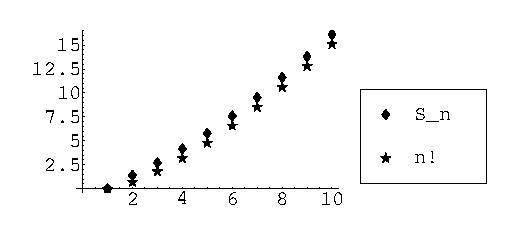
\includegraphics{Perms_gr1.eps}
\end{center}


The plot suggests that the ratio of $S_n$ and $n!$ converges to a constant, and a little experimentation, in lieu of analytical proof, reveals that constant to be $e=2.71828...$ In other words, as $n$ gets larger, $S_n$ approaches $e\times n!$, a convenient factoid.


Recall the imaginary dictionary containing an infinite number of alphabetically arranged subsections, each infinite in length. This dictionary was a mental image of the monoid of \emph{lists} of alphabetical characters, also known as the monoid of character strings under list concatenation.  Should we artificially limit the size of words in such a dictionary, we would no longer have a monoid, because the limited dictionary would not be closed under concatenation. But, we \emph{can} build a finite dictionary out of permutations. Such a dictionary would have the stupendous size $$1+S_{26}=1,096,259,850,353,149,530,222,034,277$$
ignoring differences between upper and lower case. This is a little larger than 1 billion billion billion. To set an intuition of the magnitude of this number, it is approximately the number of kilograms in the mass of the Earth. But it is finite.


Of course, this dictionary would suffer from the limitation that no duplicate letters would be permitted. This limitation is easily relieved, again in a finite fashion. Suppose we decide that words with more than four instances of a given letter are not interesting. Then, we can augment our alphabet, the type set $\T$, with three additional copies of each letter, artificially distinguished from one another by a subscript:
\[
 \{a,b,\ldots,z\}\rightarrow\{a_1,a_2,a_3,a_4,
 b_1,b_2,b_3,b_4,
 \ldots,z_1,z_2,z_3,z_4\}
\]
This device is just an application of \emph{disjoint union} from set theory. Now, our dictionary will have words with repeated letters, and will be of the more stupendous size:
\[
  1+S_{104}\approxeq 2.8\times 10^{166}
\]
which is approximately the square of the number of electrons in the observable Universe. So, while this new dictionary is technically finite, and is vastly smaller than Borges' library, it could never be physically written down, so, it is purely conceptual, once again.


The design of $\boxplus$ opens up a can of worms of practical ramifications. A computer program implementing the operation for idempotent collection monoids must have a way of detecting whether a candidate element is already in a collection. The straightforward linear search --- iterating over the entire collection --- is only practical for small collections. Other search structures, like hash tables or B-trees, are a practical necessity in any scalable implementation.


The non-idempotent (infinite) collection monoids do not escape scot-free. If they are unordered, they must also have search optimizations, not for insertion, but for finding and grouping. Only lists can scalably perform both insertion and finding, at least finding-by-numerical-index, without search optimizations (though scalable finding requires array implementation with other ramifications on recursive programming patterns).


Let us round out the zoo of collection monoids with the following definitions:


\begin{definition}
  A \textbf{set} is an unordered, idempotent collection of zero or more items of some type $\T$. A monoid of sets has the associative, commutative, recursively idempotent, binary operation, $\cup$, for combining sets, and the empty set, $\{\}=\emptyset$, for identity.
\end{definition}


Just as a monoid of permutations can be finite, so can a monoid of sets. Again, suppose a base type set $\T$ with $n$ elements. The number of elements of a set monoid drawn from $\T$ is the sum of the number of sets of length $m$ for all $m\geq 0$ to $m\leq n$. The number of sets of length $m$ turns out to be
\[
  \frac{n!}{(n-m)! m!}\defeq \binom{n}{m}
\]
which is the binomial coefficient for $n$ and $m$. This is the same as the number of permutations of length $m$ divided by $m!$ because now, the order does not matter, and there are $m!$ different ways to rearrange the elements of a permutation of length $m$. The sum of the number of sets for all $m$ is the same as the binomial $(x+y)^n$ evaluated at $x=1, y=1$. This is
\begin{align*}
  \sum_{m=0}^{n}\frac{n!}{(n-m)! m!}
  &=\binom{n}{0}+\binom{n}{1}+\cdots+\binom{n}{n-1}+\binom{n}{n}\\
  {}&{}\\
  =(x+y)^n\vert_{x=1,y=1}&=2^n
\end{align*}
Another way of seeing the result is that each set in the monoid is the result of independently choosing whether to include each element of $\T$. Since for each element of $\T$, there are two independent choices --- to include or not --- and there are $n$ elements of $\T$, there must be exactly $2^n$ sets. The monoid is just the \emph{power set} of $\T$, that is, the set of all subsets of $\T$.


To relate this to databases, consider a set of employees:
\begin{center}
\begin{tabular}{l}
  \verb"John Smith"\\
  \verb"Jean Green"\\
  \verb"Joe Snow"
\end{tabular}
\end{center}
Think of this set as a type set, $\T$, and think of the monoid of sets drawn from this type set. This monoid would be the collection of all subsets of $\T$ --- the power set of $\T$, and would have eight elements. Its monoid combination operation would be set union, $\cup$. The next section of this tutorial exhibits transformations from such a monoid to others, and how such transformations effect various `database queries' over this table of employees.


We might examine the idea of a `dictionary' built from sets of characters, just as we did for lists and permutations, but this would be a boring one, since for every choice of characters, no matter what their order, there would be only one entry. Since the essence of words built of characters is order, the monoid of sets of characters would hardly rate the moniker `dictionary.'


\begin{definition}
  A \textbf{bag} or \textbf{multiset} is an unordered collection of zero or more items of some type $\T$. A monoid of bags has the associative, commutative, non-idempotent, binary operation, $\uplus$, for combining bags, and the empty bag, $\emptybag$, for identity.
\end{definition}


A bag is like a list, except that order does not matter. So, $\LBag 1, 1, 2, 3 \RBag$ is the same as $\LBag 2, 1, 3, 1\RBag$ and the same as all twenty-two other arrangements of 1, 1, 2, and 3. Just as with lists, there are no finite bag monoids other than the trivial bag monoid, which contains only the empty bag. Just as with lists, the reason is that from any two bags, we can form a larger bag by merging the two \emph{via} the bag-combination operation, $\uplus$.


\begin{observation}
All non-idempotent collection monoids are infinite.
\end{observation}


In the database context, \emph{bag} is the default type, because databases permit duplicates. So, a table of employees, without further conditioning, might look like this:
\begin{center}
\begin{tabular}{l}
  \verb"John Smith"\\
  \verb"Jean Green"\\
  \verb"John Smith"\\
  \verb"Joe Snow"
\end{tabular}
\end{center}
This table is obviously not the full monoid of bags of such names --- such a monoid is infinite. It is just a particular element of the monoid --- a particular bag of those names.


The two copies of \verb"John Smith" are most probably not an error. It would not be surprising to have two employees with the same name, but it is incumbent on the database designer to do something to distinguish them. The usual thing is to add a column containing an arbitrary but unique employee number for each employee, and then to set a \emph{database constraint} declaring that number to be a \emph{primary key} in the table. This is an operational constraint that must be maintained at run time, incurring computational cost, as discussed above. It effectively transforms the \emph{bag} of employees to a \emph{set} of employees through a device equivalent to the disjoint union, also discussed above. There is much more about such transformations in the next section of this tutorial, but, suffice it to say, while \emph{bag} is the default in databases, \emph{set} is quite often the desired behavior.


\subsection{\color{red}Summary}


The following tables summarize everything established so far and submits a few more non-collection samples for your consideration ($\mathbb{Z}$ is the set of all integers, positive, negative, and zero; in the last column of the second table, C and I stand for commutative and idempotent, respectively). While perusing the tables, remember that, especially in the case of the collection monoids, the interpretation of the definition of a monoid, ``$\Mon{\T}{\oplus}{\Z}$ \ldots a set of elements of type $\T$ \ldots'', must include subjecting the elements of $\T$ to the unit function to bring them into the monoid as singletons.


\begin{center}
\begin{tabular}{|l|l|}
  \hline
  $\Mon{\nats}{+}{0}$ & Natural numbers under addition only \\ \hline
  $\Mon{\nats}{\times}{1}$ & Natural numbers under multiplication only \\ \hline
  $\Mon{\nats}{\max_{\nats}}{0}$ & Natural numbers with a binary \emph{max} operation \\ \hline
  $\Mon{\nats\cup\{\infty\}}{\min_{\nats}}{\infty}$ & Natural numbers and Infinity with a binary \emph{min} operation \\ \hline
  $\Mon{\ints\cup\{-\infty\}}{\max_{\ints}}{-\infty}$ & All whole numbers and
  --Infinity \& binary \emph{max} operation \\ \hline
  $\Mon{\ints\cup\{\infty\}}{\min_{\ints}}{\infty}$ & All whole numbers and
  Infinity \& binary \emph{min} operation \\ \hline
  $\Mon{\mathrm{bool}}{\lor}{\mathrm{false}}$ &
  The set $\mathrm{bool}=\{\mathrm{true},\mathrm{false}\}$ with logical \emph{or} operation, $\lor$\\ \hline
  $\Mon{\mathrm{bool}}{\land}{\mathrm{true}}$ &
  The set bool with logical \emph{and} operation, $\land$ \\ \hline
	\hline
  $\Mon{\T}{\pp}{\emptylist}$ & lists of elements that are of type $\T$ \\ \hline
  $\Mon{\T}{\boxplus}{\emptyperm}$ & permutations of elements that are of type $\T$ \\ \hline
  $\Mon{\T}{\cup}{\emptyset}$ & sets of elements that are of type $\T$ \\ \hline
  $\Mon{\T}{\uplus}{\emptybag}$ & bags of elements that are of type $\T$ \\ \hline
\end{tabular}
\end{center}


Notice that the operation, alone, suffices to identify each kind of monoid. In later sections, we may feel free to abbreviate the notation by saying, for instance, that $\boxplus$ denotes a monoid of permutations or that $\lor$ denotes the \emph{or} monoid.


\begin{center}
		\begin{tabular}{|l|l||c||c|c|c|}
		  \hline monoid &
		  singleton type   & $\oplus$        & $\Z$  & $U$         & C/I \\
		      \hline \hline
		  $\Mon{\nats}{+}{0}$ &
		  $\nats$     & $+$             & 0              &
		      $\mathrm{id}=\lambda x.x$                            & C  \\ \hline
		  $\Mon{\nats}{\times}{1}$ &
		  $\nats$     & $\times$        & 1              &
		      $\mathrm{id}$                                        & C  \\ \hline
		  $\Mon{\nats}{\max_{\nats}}{0}$ &
		  $\nats$                 & $\max_{\nats}$   & 0           &
		      $\mathrm{id}$                                        & CI \\ \hline
		  $\Mon{\nats\cup\{\infty\}}{\min_{\nats}}{\infty}$ &
		  $\nats\cup\{\infty\}$   & $\min_{\nats}$   & $\infty$    &
		      $\mathrm{id}$                                        & CI \\ \hline
		  $\Mon{\ints\cup\{-\infty\}}{\max_{\ints}}{-\infty}$ &
		  $\ints\cup\{-\infty\}$  & $\max_{\ints}$   & $-\infty$   &
		      $\mathrm{id}$                                        & CI \\ \hline
		  $\Mon{\ints\cup\{\infty\}}{\min_{\ints}}{\infty}$ &
		  $\ints\cup\{\infty\}$   & $\min_{\ints}$   & $\infty$    &
		      $\mathrm{id}$                                        & CI \\ \hline
		  $\Mon{\mathrm{bool}}{\lor}{\mathrm{false}}$ &
		  bool & $\lor$          & false    & $\mathrm{id}$ & CI \\ \hline
		  $\Mon{\mathrm{bool}}{\land}{\mathrm{true}}$ &
		  bool & $\land$         & true     & $\mathrm{id}$ & CI \\ \hline
		  \hline
		  lists &
		  $[\T]$            & $\pp$      & $\emptylist$ &
		      $\lambda x.[x]$                        & neither \\ \hline
		  permutations &
		  $\LPerm \T\RPerm$ & $\boxplus$ & $\emptyperm$ &
		      $\lambda x.\LPerm x\RPerm$ &I\\ \hline
		  sets &
		  $\{\T\}$          & $\cup$     & $\{\}=\emptyset$  &
		      $\lambda x.\{x\}$                      & CI \\ \hline
		  bags &
		  $\LBag \T\RBag$   & $\uplus$   & $\emptybag$  &
		      $\lambda x.\LBag x\RBag$               & C\\ \hline
		\end{tabular}
\end{center}


Here is another table that categorizes the kinds of collection monoids, making it obvious why there are just four kinds:


\begin{center}
  \begin{tabular}{|l||c|c|}
  \hline
  \mbox{}       & \textbf{idempotent} & \textbf{not idempotent}  \\ \hline \hline
  \multirow{2}{*}{\textbf{commutative}}
                           & set               & bag             \\
  \mbox{}                  & $\{\T\}$          & $\LBag \T\RBag$ \\ \hline
  \multirow{2}{*}{\textbf{not commutative}}
                           & permutation       & list            \\
  \mbox{}                  & $\LPerm \T\RPerm$ & $[\T]$          \\ \hline
  \end{tabular}
\end{center}


Another effective way to look at this information is as follows:
\[
\xymatrix
{
                                   & bag\ar[dr]^{idem}  &     \\
  list\ar[ur]^{comm}\ar[dr]_{idem} &                    & set \\
                                   & perm\ar[ur]_{comm} &     \\
}
\]


\emph{List} is the most primitive kind of collection monoid, because it has neither of the qualifications of commutativity (order-independence) or idempotency (lack of duplicates). Add commutativity to a list monoid, and get a bag monoid. Add idempotency to a bag monoid, get a set monoid. Add idempotency to a list monoid, get a permutation monoid. Add commutativity to a permutation monoid, get a set monoid. Add both commutativity and idempotency to a list monoid, by either pathway, get a set monoid.


And the final way to look at it is to say the two kinds of commutative collection monoid are \emph{set} and \emph{bag} and the two kinds of idempotent collection monoid are \emph{set} and \emph{permutation}.


As another abbreviation, it can be convenient to denote the types or kinds of collection monoids using just the type symbols for their singleton elements, namely $[\T]$, $\pmx{\T}$, $\{\T\}$, and $\LBag\T\RBag$, and to write $(\T)$ to be a generic catch-all symbol meaning any of the four kinds of collection monoid. This abbreviation does run the risk of confounding the type of a collection monoid with the type of the subset containing just singleton members, but at this point, we hope the distinction is so familiar that the overloading of the type symbol does not cause heartburn. We feel free to use these abbreviations in the sequel.
